% !TeX root = resume.tex

\documentclass[10pt, a4paper]{article}

\usepackage[russian]{babel}
\usepackage[utf8]{inputenc}

\usepackage{trimclip}
\usepackage{fontspec} % Для работы с системными шрифтами (нужен XeLaTeX или LuaLaTeX)
\usepackage{geometry} % Для настройки полей страницы
\usepackage{graphicx} % Для вставки изображений
\usepackage[svgnames]{xcolor} % Для работы с цветами
\usepackage[hidelinks]{hyperref}   % для кликабельных ссылок
\usepackage{enumitem}   % для настройки списков
\usepackage{fontawesome5} % Для иконок (email, телефон и т.д.)
\usepackage{tikz}       % для рисования графических элементов (линия времени, кружки)
\usetikzlibrary{shapes.misc, positioning, arrows.meta}
\usepackage{changepage}

% --- НАСТРОЙКИ ШАБЛОНА ---

% 1. ГЕОМЕТРИЯ СТРАНИЦЫ
\geometry{
    a4paper,
    left=1.5cm,
    right=1.5cm,
    top=1.5cm,
    bottom=1.5cm,
    footskip=.5cm
}



% 2. ЦВЕТА
\definecolor{maintext}{HTML}{333333} % Основной цвет текста
\definecolor{graytext}{HTML}{666666} % Серый цвет для дат и подписей
\definecolor{boxgray}{HTML}{EBEBEB}  % Цвет для "таблеток" в интересах

% 3. ШРИФТЫ
\setmainfont{Lato} % Используем шрифт Lato. Убедитесь, что он установлен
\color{maintext}
\pagestyle{empty} % Убираем нумерацию страниц

% 4. НАСТРОЙКИ ССЫЛОК
\hypersetup{
    colorlinks=true,
    urlcolor=maintext,
    linkcolor=maintext,
    pdfborder={0 0 0}, % убираем рамку вокруг ссылок
}

\setlength{\parindent}{0pt}


\begin{document}
% !TeX root = ../resume.tex

% --- ВСПОМОГАТЕЛЬНЫЕ КОМАНДЫ ---

% Команда для заголовков секций (WORK EXPERIENCE, SKILLS и т.д.)
\newcommand{\sectiontitle}[1]{%
    \vspace{8pt}
    \par
    \noindent\MakeUppercase{#1}
    \hrule width 1\textwidth height 0.4pt
    \vspace{8pt}
}

% Команда для иконки внешней ссылки
\newcommand{\extlink}{\, \textcolor{graytext}{\faIcon{external-link-alt}}}

% Команда для пунктов в списке достижений
\setlist[itemize,1]{label=\,--, leftmargin=*, topsep=0pt, itemsep=4pt}

% Команда для описания языков
\newcommand{\languageskill}[2]{%
    \par\noindent\hangindent=1em\hangafter=0
    \makebox[8em][l]{#1} % Название языка
    \foreach \i in {1,...,5}{
        \ifnum\i > #2
            \tikz\draw[graytext, fill=white] (0,0) circle (2.5pt);
        \else
            \tikz\fill[maintext] (0,0) circle (2.5pt);
        \fi
        \hspace{2pt}
    }
    \vspace{4pt}
}

% Команда для "таблеток" с интересами
\newcommand{\interesttag}[1]{%
    \tikz[baseline=(X.base)] \node[draw=graytext, rounded corners=3pt, inner sep=4pt, text=graytext] (X) {#1};
}

% ===============================================================
% ШАПКА (ИМЯ, ФОТО, КОНТАКТЫ)
% ===============================================================

\begin{minipage}[t]{0.6\textwidth} % Левая часть шапки
    \begin{minipage}[c]{0.25\textwidth}
        \begin{tikzpicture}
            \clip (0,0) rectangle (\linewidth, \linewidth); % Определяем область видимости (квадрат)
            \node[
                inner sep=0pt, % убираем внутренние отступы
                path picture={
                    \node[
                        xshift=0, % сдвигаем фото влево
                        yshift=-30pt, % сдвигаем фото вверх
                    ] at (path picture bounding box.center) {
                        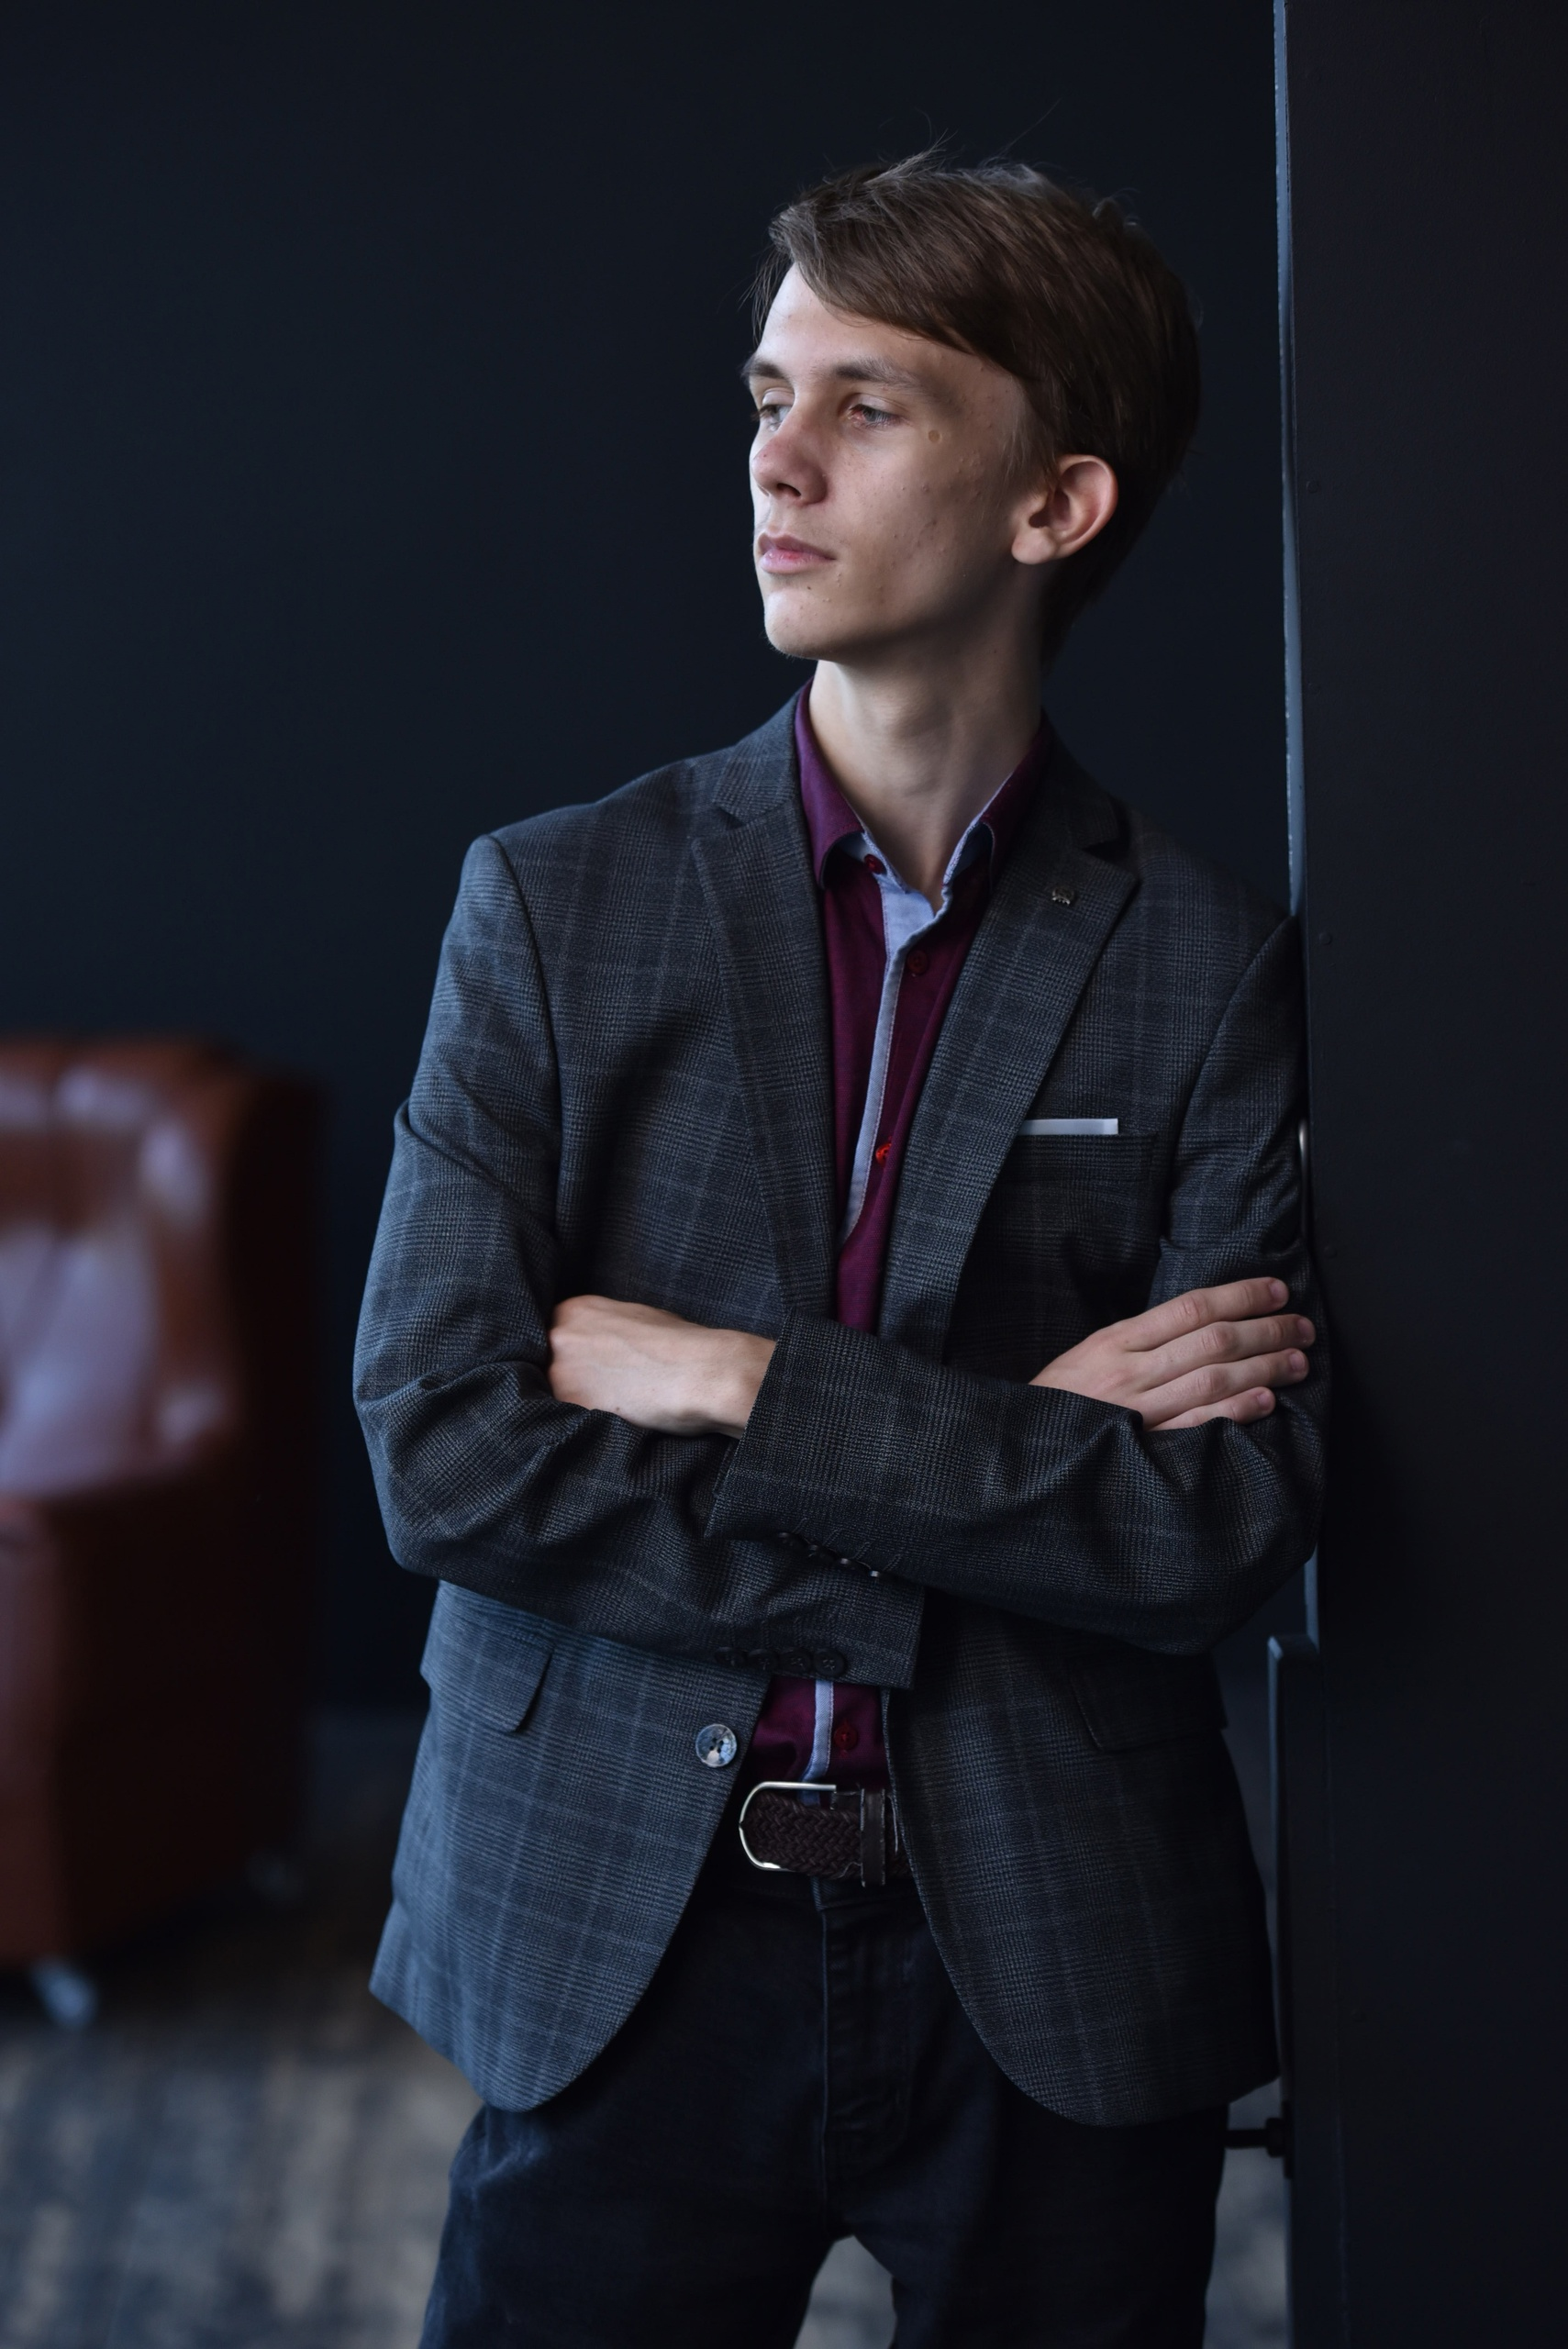
\includegraphics[width=1.2\linewidth]{pics/self-photo.jpg}; % вставляем фото
                    };
                }
            ] at (0.5\linewidth, 0.5\linewidth) [draw=none, fill=none, minimum width=\linewidth, minimum height=\linewidth, rounded corners=15pt] {};
            % Рисуем рамку с закругленными углами, если нужно
            \draw[rounded corners=15pt] (0,0) rectangle (\linewidth, \linewidth);
        \end{tikzpicture}
    \end{minipage}%
    \hspace{0.02\textwidth} % Отступ между фото и текстом
    \begin{minipage}[c]{0.7\textwidth}
        \Huge \textbf{Новиков} \\
        \Huge \textbf{Сергей} \\
        \Huge \textbf{Александрович}
    \end{minipage}
\end{minipage}%
\begin{minipage}{0.4\textwidth} % Правая часть шапки
    \raggedleft
    \small
    \href{tel:+79635716695}{+7 (963) 571-66-95} \faIcon{mobile-alt} \\[4pt]
    \href{mailto:isnov.contact@gmail.com}{isnov.contact@gmail.com} \faEnvelope \\[4pt]
    \href{https://t.me/Isn0v}{@Isn0v} \faIcon{telegram-plane} \\[4pt]
    \href{https://m.vk.com/isn0v}{vk.com/isn0v} \faIcon{vk} \\[4pt]
    \href{https://github.com/Isn0v}{github.com/Isn0v} \faIcon{github} \\[4pt]
    \href{https://leetcode.com/u/Isn0v/}{leetcode.com/Isn0v} \faIcon{code} \\[4pt]
\end{minipage}

\vspace{1cm}

% ===============================================================
% КРАТКАЯ СВОДКА (SUMMARY)
% ===============================================================

\raggedright
Программист с опытом работы в комманде. Во время своего обучения разрабатывал проекты вместе с одногрупниками, иногда брав на себя ответственность в организации. Есть опыт разработки на C/C++, Go, Python. Активно изучаю компьютерные сети и DevOps инструменты и применяю эти знания на парктике, в своих проектах. Есть промышленный опыт работы с GitLab CI. Быстро осваиваю новые технологии и умею эффективно взаимодействовать с командой без каких-либо проблем и конфликтов.
\newline
\newline
C Сентября по Январь 2025 занимался исследовательской деятельностью в \textbf{Excelsior at Huawei}, посвященной изучению устройства ОС Linux, а именно устройства процессов, файловой системы, планировщика, архитектуры и механизмов для изоляции и манипуляции ресурсами ОС. Позже перешел в штат.


% ===============================================================
% ДВУХКОЛОНОЧНАЯ СТРУКТУРА
% ===============================================================

% Создаем две колонки: левая 70% ширины, правая 30%
\begin{minipage}[t]{0.55\textwidth}

\raggedright

% --- ОПЫТ РАБОТЫ ---
\sectiontitle{\faBriefcase \quad Опыт работы}
\begin{tikzpicture}[remember picture]
    \node[circle, fill=maintext, inner sep=2.5pt] (c1) at (0,0) {};
\end{tikzpicture}
\hspace{0.5cm}
\begin{minipage}[t]{0.9\textwidth}
    \raggedright
    \textbf{\Large DevOps Инженер} \\[2pt]
    \textcolor{graytext}{\href{https://rnew.tilda.ws/excelsiorathuawei}{Excelsior at Huawei}}\extlink \\
    \textcolor{graytext}{\textit{02/2025 - 07/2025}}
    \begin{itemize}
        \item \textbf{Разрабатывал} и внедрял новые функции в существующие GitLab CI/CD конвейеры.
        \item \textbf{Оптимизировал} структуру конвейера для уменьшения времени выполнения и улучшения стабильности.
        \item \textbf{Улучшал} читаемость и поддерживаемость конфигураций.
        \item \textbf{Документировал} все изменения и предоставленные функции.
    \end{itemize}
\end{minipage}

\vspace{1cm}

\sectiontitle{\faFolderOpen \quad Проекты}
\begin{tikzpicture}[remember picture]
    \node[circle, fill=maintext, inner sep=2.5pt] (c1) at (0,0) {};
\end{tikzpicture}
\hspace{0.5cm}
\begin{minipage}[t]{0.9\textwidth}
    \raggedright
    \textbf{\Large \href{https://github.com/Isn0v/gemini-gateway}{Gemini-Gateway}\extlink } \\[2pt]
    Небольшой клиент-серверный проект, где сервер - шлюз между \textbf{Gemini AI API} и пользователем, а клиент - сам пользователь, который отправляет запросы через этот шлюз. Цель проекта заключается в познании логики работы с таким стеком технологий, как Kubernetes, Helm, Prometheus, Grafana. Другими словами, DevOps инструментами.\\
\end{minipage}

\vspace{0.5cm}

\begin{tikzpicture}[remember picture]
    \node[circle, fill=maintext, inner sep=2.5pt] (c1) at (0,0) {};
\end{tikzpicture}
\hspace{0.5cm}
\begin{minipage}[t]{0.9\textwidth}
    \raggedright
    \textbf{\Large \href{https://github.com/B0GDANPN/BrickOS/tree/main}{BrickOS}\extlink}  \\[2pt]
    Упрощенная реализация ядра операционной системы с обработкой прерываний на C и Assembler\\
\end{minipage}

\vspace{0.5cm}

\begin{tikzpicture}[remember picture]
    \node[circle, fill=maintext, inner sep=2.5pt] (c1) at (0,0) {};
\end{tikzpicture}
\hspace{0.5cm}
\begin{minipage}[t]{0.9\textwidth}
    \raggedright
    \textbf{\Large \href{https://github.com/VolkovK04/NSTTF}{NSTTF (Not So Tiny Tensorflow)}\extlink}  \\[2pt]
    Упрощенная реализация Tensorflow на C++ с поддержкой ускорения на GPU \\
\end{minipage}

\vspace{0.5cm}


% --- ОБРАЗОВАНИЕ ---

\end{minipage}%
\hfill % Разделитель между колонками
\begin{minipage}[t]{0.4\textwidth}

\sectiontitle{\faGraduationCap \quad Образование}
% \hspace{0.5cm}
\begin{minipage}[t]{\textwidth}
    \raggedright
    \textbf{\Large Математика и \\Компьютерные Науки} \\[2pt]
    \textit{\large \href{https://sys.pro/}{Системное Программирование} \extlink} \\[4pt]
    \textcolor{graytext}{Новосибирский Государственный Университет} \\
    \textcolor{graytext}{\textit{Механико Математический факультет, \\Бакалавр},\\ \textit{2022 - 2026}}
\end{minipage}

\vspace{0.5cm}

% --- НАВЫКИ ---
\sectiontitle{\faCog \quad Навыки}
\begin{minipage}[t]{0.5\textwidth}
    \raggedright
    \small
    Linux \\[4pt]
    Алгоритмы и Структуры данных \\[4pt]
    GitLab CI/CD \\[4pt]
    Git \& GitHub \\[4pt]
    C, C++, Go, Python \\[4pt]
    Компьютерные сети \\[4pt]
    Docker, K8s \\[4pt]
    Grafana, Prometheus \\[4pt]
    ELK
\end{minipage}%
\hfill
\begin{minipage}[t]{0.5\textwidth}
    \raggedleft
    \small
    Адаптируемость \\[4pt]
    Ответственность \\[4pt]
    Работа в комманде \\[4pt]
    Неконфликтность \\[4pt]
\end{minipage}

\vspace{0.5cm}

% --- ЯЗЫКИ ---
\sectiontitle{\faGlobe \quad Языки}
% \small
% \languageskill{Русский}{5}
% \languageskill{Английский}{4}
Русский \\[4pt]
Английский


\end{minipage}

\end{document}